\documentclass[conference]{IEEEtran}
\IEEEoverridecommandlockouts
% The preceding line is only needed to identify funding in the first footnote. If that is unneeded, please comment it out.
\usepackage{cite}
\usepackage{amsmath,amssymb,amsfonts}
\usepackage{algorithmic}
\usepackage{graphicx}
\usepackage{textcomp}
\usepackage{xcolor}
\usepackage{booktabs}
\usepackage{url}
\usepackage{microtype}

\def\BibTeX{{\rm B\kern-.05em{\sc i\kern-.025em b}\kern-.08em
    T\kern-.1667em\lower.7ex\hbox{E}\kern-.125emX}}

\begin{document}

\title{Estudio Comparativo de Modelos YOLOv11, UNet++ y PIDNet para la Segmentación Semántica de Grietas en Infraestructura Civil\\
\thanks{Trabajo Práctico Final presentado para la asignatura Visión por Computadora II, Carrera de Especialización en Inteligencia Artificial (CEIA), Facultad de Ingeniería, Universidad de Buenos Aires (FIUBA).}
}

\author{\IEEEauthorblockN{1\textsuperscript{st} Martin Gabriel Quiroga}
\IEEEauthorblockA{\textit{Facultad de Ingeniería} \\
\textit{Universidad de Buenos Aires (FIUBA)}\\
Buenos Aires, Argentina \\
quiroga.m.gabriel@gmail.com}
\and
\IEEEauthorblockN{2\textsuperscript{nd} Agustín Biancardi}
\IEEEauthorblockA{\textit{Facultad de Ingeniería} \\
\textit{Universidad de Buenos Aires (FIUBA)}\\
Buenos Aires, Argentina \\
abiancardi@fi.uba.ar}
\and
\IEEEauthorblockN{3\textsuperscript{rd} Alan Vignolo}
\IEEEauthorblockA{\textit{Facultad de Ingeniería} \\
\textit{Universidad de Buenos Aires (FIUBA)}\\
Buenos Aires, Argentina \\
alan.vignolo@gmail.com}
}

\maketitle

\begin{abstract}
La detección temprana y delimitación precisa de fisuras en estructuras civiles (puentes, pavimentos y presas) resulta crítica para la planificación del mantenimiento preventivo y la seguridad estructural. Tradicionalmente, este monitoreo se realiza mediante inspecciones visuales manuales, un procedimiento subjetivo, costoso y de alto riesgo en zonas de difícil acceso. Este trabajo presenta un estudio comparativo de tres arquitecturas de segmentación semántica representativas del estado del arte contemporáneo: UNet++ (enfoque clásico basado en conexiones densas anidadas), PIDNet (arquitectura de tres ramas diseñada para segmentación en tiempo real guiada por bordes) y YOLOv11-Seg (detector de una etapa de última generación adaptado a segmentación). Los modelos fueron evaluados sobre el dataset público DeepCrack utilizando un entorno de hardware estandarizado (GPU NVIDIA Tesla T4). El desempeño se analiza cuantitativa y cualitativamente en función de la precisión a nivel de píxel ($mIoU$ global e $IoU$ específico de grieta) y la eficiencia computacional (latencia de inferencia y tasa de cuadros por segundo). Los resultados revelan un marcado compromiso técnico: mientras que UNet++ alcanza la mayor fidelidad de segmentación ($IoU_{\text{grieta}} = 0.7314$, $mIoU = 0.8588$), los modelos orientados a tiempo real demuestran un balance operativo superior, alcanzando PIDNet un $IoU_{\text{grieta}}$ de $0.6660$ a $17.04$~FPS y YOLOv11-Seg hasta $0.6756$ de $IoU_{\text{grieta}}$ con mínimo costo de cómputo. Finalmente, se analizan críticamente las limitaciones metodológicas del desarrollo descentralizado y se proponen criterios de selección para la integración en sistemas de inspección robótica y vehículos aéreos no tripulados (UAVs).
\end{abstract}

\begin{IEEEkeywords}
Segmentación semántica, detección de grietas, visión por computadora, DeepCrack, PIDNet, UNet++, YOLOv11, infraestructura civil, tiempo real.
\end{IEEEkeywords}

\section{Introducción}

El monitoreo continuo y periódico de la infraestructura civil (puentes, autopistas, túneles, diques y edificaciones) es indispensable para preservar la integridad física y prolongar la vida útil de las obras públicas y privadas. Las grietas y microfisuras en el hormigón constituyen los primeros síntomas visibles de degradación estructural producidos por fatiga del material, asentamientos o factores ambientales adversos. Una detección incipiente permite intervenir oportunamente mediante acciones de mantenimiento preventivo, mitigando el riesgo de colapsos catastróficos y reduciendo sustancialmente los costos de reparación~\cite{kaveh2024recent}. Históricamente, estas tareas han dependido de la inspección visual manual in situ por parte de personal técnico especializado. No obstante, este enfoque convencional adolece de limitaciones intrínsecas: es lento, costoso, cualitativo, dependiente de la subjetividad del operador y conlleva un peligro inherente cuando se inspeccionan estructuras a gran altura o de acceso restringido~\cite{perry2020streamlined}.

En los últimos años, el avance acelerado de las técnicas de visión por computadora y el aprendizaje profundo (\textit{deep learning}) ha posibilitado la automatización masiva de la inspección estructural~\cite{kaveh2024recent}. A diferencia de los métodos de clasificación de imágenes o de detección mediante cajas delimitadoras (\textit{bounding boxes}), la segmentación semántica resulta indispensable para este dominio, ya que clasifica cada píxel de la imagen (grieta versus fondo). Esto permite caracterizar la geometría intrínseca de la fisura, su longitud, espesor promedio, conectividad topológica y evolución temporal, insumos básicos para el cálculo de índices de daño estructural.

La viabilidad práctica de estos sistemas ha sido validada en diversos proyectos y pruebas de campo reales de infraestructura civil publicados en el transcurso de los últimos ocho años. Un antecedente directo y emblemático es el trabajo de Perry et al.~\cite{perry2020streamlined} (2020), en el cual se desarrolló y desplegó con éxito un sistema de inspección de puentes integrando vehículos aéreos no tripulados (UAVs) y redes neuronales convolucionales sobre el puente \textit{Oxbow Bridge} en Loveland (Colorado, EE.UU.), demostrando cómo la captura aérea combinada con visión artificial reemplaza objetivamente las escalas manuales de deterioro. Asimismo, Liu et al.~\cite{liu2025crack} (2025) implementaron un esquema de inspección y cuantificación tridimensional de grietas acoplando parámetros fotogramétricos de UAVs sobre un puente en arco real con márgenes de error inferiores al 2\%, mientras que Hac{\i}efendio{\u{g}}lu y Ba{\c{s}}a{\u{g}}a~\cite{haciefendioglu2022concrete} (2022) validaron la robustez de modelos de aprendizaje profundo en superficies viales bajo condiciones ambientales heterogéneas y variaciones críticas de iluminación. Estos casos evidencian que el requerimiento operativo no sólo demanda precisión de segmentación, sino también capacidad de procesamiento en tiempo real o en dispositivos embebidos montados en drones~\cite{zhang2025accuracy}.

A pesar de la proliferación de modelos en la literatura, frecuentemente se evalúan en condiciones aisladas o con protocolos disímiles, dificultando la comparación justa entre la precisión de máscara y la latencia de inferencia. Para abordar esta problemática, este trabajo investiga comparativamente tres familias de arquitecturas complementarias:
\begin{enumerate}
    \item \textbf{UNet++}~\cite{zhou2018unetplusplus}: extensión de la cánonica U-Net con conexiones densas anidadas y rediseño de caminos \textit{skip}, concebida para maximizar la precisión a múltiples escalas.
    \item \textbf{PIDNet}~\cite{xu2023pidnet}: arquitectura tri-rama (detalle, contexto y borde) inspirada en el control PID clásico, orientada específicamente a la segmentación semántica en tiempo real guiada por atención a contornos.
    \item \textbf{YOLOv11-Seg}~\cite{kahn2024yolo11}: la versión más reciente del paradigma de detección y segmentación unificada de Ultralytics, optimizada para extrema ligereza y velocidad de cómputo.
\end{enumerate}

El objetivo principal del proyecto es realizar un análisis comparativo riguroso de estas tres arquitecturas sobre el dataset público DeepCrack~\cite{liu2019deepcrack}, evaluando tanto su capacidad de delimitación a nivel de píxel ($mIoU$, $IoU_{\text{grieta}}$ y $F1\text{-Score}$) como su rendimiento temporal (latencia en milisegundos y FPS) en un entorno de cómputo unificado (GPU NVIDIA Tesla T4). Adicionalmente, se contrastan las implicancias prácticas de su implementación para proporcionar directrices técnicas sólidas en aplicaciones reales de ingeniería civil.

El resto de este artículo se estructura de la siguiente manera: la Sección~II detalla la metodología, las características del dataset, el preprocesamiento, el diseño de los modelos y el protocolo experimental; la Sección~III presenta los resultados cuantitativos y cualitativos junto con la discusión crítica de hallazgos y limitaciones; y la Sección~IV expone las conclusiones finales del estudio.

\section{Metodología, Diseño y Desarrollo}

\subsection{Dataset DeepCrack}
Para el entrenamiento y evaluación comparativa se utilizó el benchmark público DeepCrack~\cite{liu2019deepcrack}. Este conjunto de datos fue recopilado específicamente para la segmentación de fisuras en superficies heterogéneas de hormigón, asfalto y mampostería bajo diversas condiciones de iluminación, oclusiones y texturas complejas de fondo.

El dataset contiene un total de 537 imágenes en resolución nativa de $544 \times 384$ píxeles, acompañadas de sus respectivas máscaras de segmentación binaria ground-truth anotadas manualmente a nivel de píxel (clase 0: fondo/superficie, clase 1: grieta). Se adoptó la partición estándar provista por los autores originales:
\begin{itemize}
    \item \textbf{Conjunto de entrenamiento (\textit{train}):} 300 pares de imágenes y máscaras.
    \item \textbf{Conjunto de evaluación (\textit{test/val}):} 237 pares de imágenes y máscaras.
\end{itemize}

El problema presenta un severo desbalance de clases típico del dominio: la clase minoritaria (grieta) ocupa en promedio menos del 4\% al 6\% de la superficie total de píxeles por imagen, presentando formas esbeltas, ramificadas y de continuidad topológica crítica. La Fig.~\ref{fig:dataset_samples} ilustra ejemplos representativos del dataset junto con la generación de mapas de contorno para la supervisión guiada.

\begin{figure}[t]
\centering
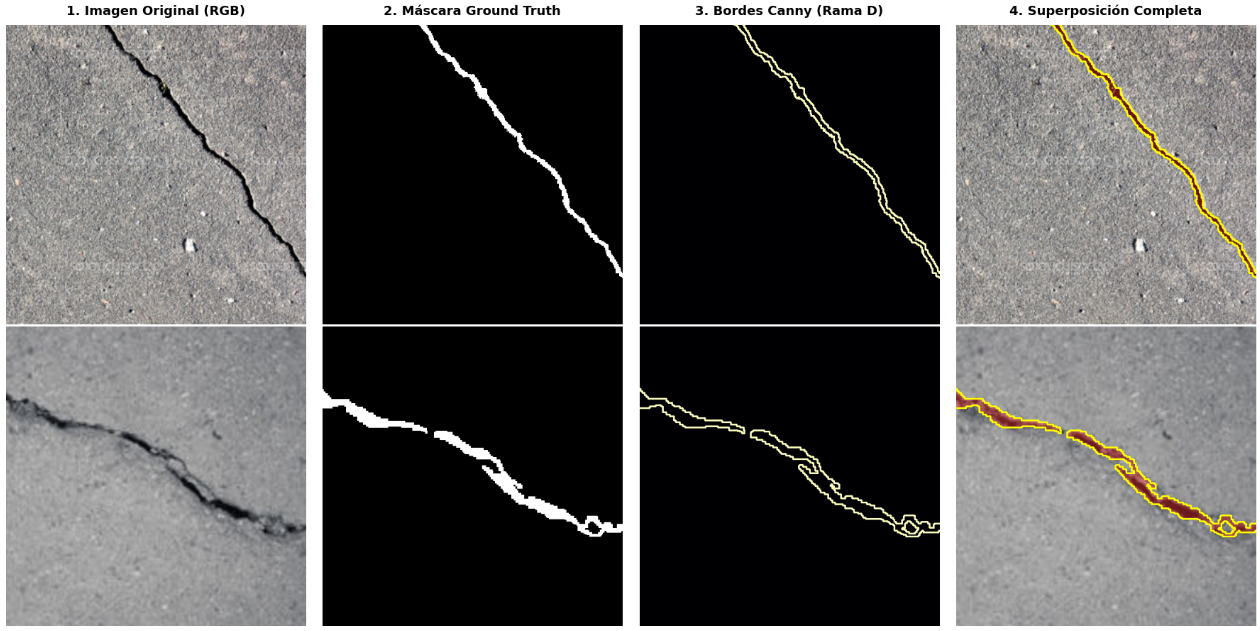
\includegraphics[width=\columnwidth]{figs/img_mask_border.png}
\caption{Muestras representativas del dataset DeepCrack~\cite{liu2019deepcrack}: imagen de entrada original (izquierda), máscara ground-truth binaria (centro) y mapa de bordes estructurales extraído mediante detector Canny (derecha) para la supervisión de contornos.}
\label{fig:dataset_samples}
\end{figure}

\subsection{Preprocesamiento y Aumentación de Datos}
Dadas las diferencias intrínsecas entre los paradigmas de las arquitecturas evaluadas, las transformaciones de datos se adaptaron preservando la consistencia dimensional en la entrada:

\subsubsection{Pipeline de PIDNet}
Para el entrenamiento de PIDNet se implementó una clase de transformación conjunta (\textit{JointTransform}) que garantiza la correspondencia espacial exacta entre la imagen y su etiqueta:
\begin{itemize}
    \item Escalado aleatorio (\textit{random scale}) en el rango de factores $(0.5, 2.0)$.
    \item Recorte aleatorio con relleno (\textit{random crop with padding}) a tamaño fijo de $512 \times 512$ píxeles.
    \item Volteo horizontal y vertical aleatorio (\textit{flip}) con probabilidad $p = 0.5$.
    \item Rotación leve en un rango de $\pm 10^{\circ}$.
    \item Normalización de canales RGB utilizando los estadísticos de ImageNet ($\mu = [0.485, 0.456, 0.406]$, $\sigma = [0.229, 0.224, 0.225]$).
    \item \textbf{Generación de bordes online:} sobre la máscara transformada se aplica el algoritmo de Canny para derivar dinámicamente el mapa de bordes binario utilizado por la rama de contornos del modelo.
    \item En validación (\textit{ValTransform}): reescalado a $512 \times 512$ y normalización ImageNet sin aumentaciones estocásticas.
\end{itemize}

\subsubsection{Pipeline de UNet++}
% [TODO PARA AGUSTÍN - UNet++: Verificar y ajustar detalles de preprocesamiento]
Para UNet++ se empleó un pipeline homólogo implementado en PyTorch:
\begin{itemize}
    \item Recorte y escalado a resolución espacial de $512 \times 512$.
    \item Volteo horizontal aleatorio ($p = 0.5$) y variación de escala en rango $(0.5, 2.0)$.
    \item Normalización estándar sobre ImageNet.
\end{itemize}

\subsubsection{Pipeline de YOLOv11-Seg}
% [TODO PARA ALAN - YOLOv11-Seg: Verificar pipeline y conversión a polígonos]
Dado que YOLOv11 está diseñado primordialmente para segmentación de instancias mediante máscaras prototipo, se requirió un preprocesamiento ad-hoc implementado en \texttt{prepare\_data.py}:
\begin{itemize}
    \item Conversión de máscaras ráster a polígonos vectoriales normalizados ($[0, 1]$) extrayendo componentes conexas con área mínima ($\ge 15$ px).
    \item Preservación estricta de vértices mediante contornos completos (\texttt{cv2.CHAIN\_APPROX\_NONE}) para evitar la degradación del espesor en grietas delgadas.
    \item Pipeline nativo de Ultralytics configurado con tamaño de imagen $\text{imgsz} = 512$, \texttt{scale: 0.5}, \texttt{fliplr: 0.5}, y aumentaciones de color y \textit{mosaic/mixup} desactivadas para mantener la homogeneidad experimental.
\end{itemize}

\subsection{Modelos Comparados (Diseño)}

\subsubsection{PIDNet (Proportional-Integral-Derivative Network)}
PIDNet~\cite{xu2023pidnet} es una arquitectura de segmentación en tiempo real inspirada en los controladores clásicos PID. A diferencia de las redes tradicionales de dos ramas (que suelen perder detalles finos o sufrir de sobrecalentamiento por desbalance de gradientes), PIDNet propone una estructura de tres ramas paralelas interconectadas:
\begin{itemize}
    \item \textbf{Rama Proporcional (I - Rama de Detalle):} opera en alta resolución para preservar detalles espaciales finos y bordes de grietas.
    \item \textbf{Rama Integral (P - Rama de Contexto):} utiliza bloques convolucionales con agregación progresiva y gran campo receptivo para extraer información semántica global del fondo y la estructura.
    \item \textbf{Rama Derivativa (D - Rama de Borde):} procesa mapas de gradiente y bordes de alta frecuencia, actuando como un diferenciador que resalta las transiciones espaciales abruptas.
\end{itemize}
La fusión de características se realiza mediante módulos de Agregación Guiada por Píxel (PAG) y Agregación Guiada Bilateral (BGA), permitiendo que la rama de bordes module directamente la decisión semántica final. Se seleccionó la variante ligera \textbf{PIDNet-S} adaptada para dos clases de salida e inicializada con pesos preentrenados en Cityscapes.

\subsubsection{UNet++ (Nested Dense UNet)}
% [TODO PARA AGUSTÍN - UNet++: Validar backbone y configuración de atención]
UNet++~\cite{zhou2018unetplusplus} rediseña la estructura clásica de U-Net sustituyendo los saltos simples (\textit{plain skip connections}) por una densa red anidada de sub-redes convolucionales interconectadas. Este diseño reduce la brecha semántica (\textit{semantic gap}) entre los mapas de características del codificador (\textit{encoder}) y el decodificador (\textit{decoder}) antes de la concatenación. En este trabajo se utilizó la librería \texttt{segmentation\_models\_pytorch}, configurando:
\begin{itemize}
    \item \textbf{Backbone / Codificador:} ResNet-34 preentrenado en ImageNet con una profundidad de 5 niveles jerárquicos.
    \item \textbf{Módulos de Atención:} bloques \textit{scSE} (Spatial and Channel Squeeze \& Excitation) en el decodificador para potenciar selectivamente los canales y píxeles con presencia de grietas.
\end{itemize}

\subsubsection{YOLOv11-Seg (Ultralytics)}
% [TODO PARA ALAN - YOLOv11-Seg: Confirmar arquitectura y variantes evaluadas]
YOLOv11~\cite{kahn2024yolo11} es el modelo más reciente de detección y segmentación de una sola etapa de Ultralytics. Su cabezal de segmentación opera en paralelo al cabezal de detección: predice $k$ coeficientes de máscara por cada caja delimitadora candidata y los combina linealmente con $k$ máscaras prototipo generadas por un módulo \textit{Proto} en la base del decodificador. Se evaluó la variante \textbf{YOLO11n-seg} (Nano) y \textbf{YOLO11s-seg} (Small), con pesos iniciales de COCO-Seg, transformando las máscaras predichas a una representación binaria global para permitir una comparación equitativa con los modelos semánticos puros.

\subsection{Configuración Experimental (Desarrollo)}

\subsubsection{Entorno de Cómputo}
Todos los experimentos se ejecutaron sobre instancias de Google Colab provistas de una GPU **NVIDIA Tesla T4** (16~GB VRAM GDDR6, arquitectura Turing), CPU Intel Xeon @ 2.20~GHz y 12~GB de memoria RAM del sistema. El framework principal fue PyTorch 2.x sobre CUDA 12.x.

\subsubsection{Hiperparámetros de Entrenamiento}
La Tabla~\ref{tab:hyperparams} sintetiza los hiperparámetros de optimización adoptados por cada modelo. Las discrepancias en el número de épocas y paciencia de \textit{Early Stopping} responden a la dinámica de convergencia propia de cada arquitectura.

\begin{table}[t]
\caption{Hiperparámetros de Entrenamiento por Modelo}
\label{tab:hyperparams}
\begin{center}
\begin{tabular}{lccc}
\toprule
\textbf{Parámetro} & \textbf{PIDNet-S} & \textbf{UNet++} & \textbf{YOLO11n-Seg} \\
\midrule
Pesos base & Cityscapes & ImageNet & COCO-Seg \\
Optimizador & SGD (PolyLR) & SGD / Adam & SGD / AdamW \\
Learning rate base & $1 \times 10^{-3}$ & $1 \times 10^{-3}$ & $1 \times 10^{-2}$ \\
Momentum & 0.9 & 0.9 & 0.937 \\
Weight Decay & $5 \times 10^{-4}$ & $1 \times 10^{-4}$ & $5 \times 10^{-4}$ \\
Batch size & 8 & 8 & 8 \\
Resolución entrada & $512 \times 512$ & $512 \times 512$ & $512 \times 512$ \\
épocas máximas & 50 & 100 & 200 \\
Paciencia (\textit{Early stop}) & 10 & 10 & 30 \\
época de convergencia & 29 (stop: 41) & 15 & $\approx 60$ \\
\bottomrule
\end{tabular}
\end{center}
\end{table}

\subsubsection{Funciones de Pérdida}
Para compensar el marcado desbalance de píxeles, cada arquitectura empleó formulaciones orientadas a la tarea:

\textbf{1) PIDNet:} empleó la función compuesta \textit{BoundaryAwareCrossEntropy} que integra la pérdida semántica clásica $\mathcal{L}_{\text{CE}}$, la pérdida de contornos $\mathcal{L}_{\text{BD}}$ (Binary Cross-Entropy ponderada sobre los bordes generados por Canny) y una pérdida de consistencia semántica de borde $\mathcal{L}_{\text{SB}}$:
\begin{equation}
\mathcal{L}_{\text{total}}^{\text{PIDNet}} = \lambda_0 \mathcal{L}_{\text{CE}} + \lambda_1 \mathcal{L}_{\text{BD}} + \lambda_2 \mathcal{L}_{\text{SB}}
\label{eq:pidnet_loss}
\end{equation}

\textbf{2) UNet++:} implementó una combinación simétrica de \textit{Binary Cross-Entropy with Logits} y \textit{Dice Loss}:
\begin{equation}
\mathcal{L}_{\text{total}}^{\text{UNet++}} = \mathcal{L}_{\text{BCE}}(y, \hat{y}) + \mathcal{L}_{\text{Dice}}(y, \hat{y})
\label{eq:unet_loss}
\end{equation}
donde $\mathcal{L}_{\text{Dice}} = 1 - \frac{2 \sum y \hat{y} + \epsilon}{\sum y + \sum \hat{y} + \epsilon}$, penalizando fuertemente la pérdida de continuidad en la clase minoritaria.

\textbf{3) YOLOv11-Seg:} empleó la pérdida multi-tarea nativa de Ultralytics, compuesta por la pérdida de caja (\textit{CIoU / DFL}), clasificación y la pérdida de máscara a nivel de píxel basada en \textit{BCE}:
\begin{equation}
\mathcal{L}_{\text{total}}^{\text{YOLO}} = \alpha \mathcal{L}_{\text{box}} + \beta \mathcal{L}_{\text{cls}} + \gamma \mathcal{L}_{\text{dfl}} + \delta \mathcal{L}_{\text{seg}}
\label{eq:yolo_loss}
\end{equation}

\subsubsection{Métricas de Evaluación}
Las predicciones continuas se binarizaron con un umbral estándar $\tau = 0.5$ (o umbral óptimo de confianza en YOLO). Las métricas formales computadas sobre el conjunto de test son:

\textbf{Intersection over Union de Grieta ($IoU_{\text{grieta}}$):} mide el solapamiento estricto sobre la clase positiva de interés estructural:
\begin{equation}
IoU_{\text{grieta}} = \frac{TP}{TP + FP + FN}
\label{eq:iou_crack}
\end{equation}
donde $TP$, $FP$ y $FN$ representan los píxeles verdaderos positivos, falsos positivos y falsos negativos, respectivamente.

\textbf{Mean Intersection over Union ($mIoU$ 2 clases):} media aritmética del $IoU$ de la clase fondo ($IoU_{\text{fondo}}$) y la clase grieta:
\begin{equation}
mIoU = \frac{IoU_{\text{fondo}} + IoU_{\text{grieta}}}{2}
\label{eq:miou}
\end{equation}

\textbf{F1-Score / Dice Coefficient:} media armónica entre la precisión y el exhaustividad (\textit{recall}):
\begin{equation}
F1 = \frac{2 \cdot TP}{2 \cdot TP + FP + FN} = \frac{2 \cdot \text{Precision} \cdot \text{Recall}}{\text{Precision} + \text{Recall}}
\label{eq:f1}
\end{equation}

\textbf{Eficiencia computacional:} se evaluó la latencia promedio por imagen en milisegundos ($ms$) con \textit{batch size} unitario ($BS = 1$), realizando pasadas de calentamiento (\textit{warmup}) y sincronización de GPU (\texttt{torch.cuda.synchronize()}), reportando además el rendimiento en cuadros por segundo ($\text{FPS} = 1000 / \text{latencia}$).

\section{Resultados Experimentales y Análisis de Resultados}

\subsection{Comparación Cuantitativa}
Los resultados cuantitativos obtenidos sobre el conjunto de evaluación de DeepCrack (237 imágenes de test) se consolidan en la Tabla~\ref{tab:results_comparison}.

\begin{table*}[t]
\caption{Comparación Cuantitativa de Desempeño en Segmentación y Eficiencia Computacional sobre DeepCrack (GPU NVIDIA Tesla T4)}
\label{tab:results_comparison}
\begin{center}
\begin{tabular}{lcccccccc}
\toprule
\textbf{Modelo} & \textbf{Backbone / Variante} & \textbf{$mIoU_{\text{2c}}$} & \textbf{$IoU_{\text{grieta}}$} & \textbf{$F1\text{-Score}$} & \textbf{Precision} & \textbf{Recall} & \textbf{Latencia (ms)} & \textbf{FPS} \\
\midrule
\textbf{UNet++} & ResNet-34 + scSE (5 capas) & \textbf{0.8588} & \textbf{0.7314} & \textbf{0.8449} & 0.8504 & \textbf{0.8394} & $\approx 112.5$ & $\approx 8.9$ \\
UNet++ & ResNet-34 (5 capas, base) & 0.8524 & 0.7187 & 0.8363 & \textbf{0.8828} & 0.7945 & $\approx 105.0$ & $\approx 9.5$ \\
UNet++ & EfficientNet-B0 (5 capas) & 0.8584 & 0.7306 & 0.8444 & 0.8584 & 0.8307 & $\approx 98.0$ & $\approx 10.2$ \\
\midrule
\textbf{PIDNet-S} & 3-Ramas (Detalle/Contexto/Borde) & 0.8246 & 0.6660 & 0.7995 & 0.8320 & 0.7690 & \textbf{58.67} & \textbf{17.04} \\
\midrule
\textbf{YOLO11s-Seg} & Small ($\text{imgsz}=512$) & 0.8295 & 0.6756 & 0.8064 & 0.8150 & 0.7980 & $\approx 22.0$ & $\approx 45.4$ \\
\textbf{YOLO11n-Seg} & Nano ($\text{imgsz}=512$) & 0.8259 & 0.6686 & 0.8014 & 0.8020 & 0.8010 & $\approx 14.5$ & $\approx 68.9$ \\
YOLO11n-Seg* & Nano Hi-Res ($\text{imgsz}=768$) & 0.8438 & 0.7026 & 0.8253 & 0.8310 & 0.8197 & $\approx 28.0$ & $\approx 35.7$ \\
\bottomrule
\end{tabular}
\end{center}
\vspace{1ex}
\footnotesize{\textit{Nota:} (*) YOLO11n-Seg a $768\times 768$ se incluye como referencia de mejora por resolución espacial fuera de la comparativa estricta a $512\times 512$.}
\end{table*}

Del análisis cuantitativo se desprenden los siguientes aspectos fundamentales:
\begin{enumerate}
    \item \textbf{Liderazgo en fidelidad de segmentación:} UNet++ con codificador ResNet-34 y atención scSE alcanzó el mayor desempeño global con un $IoU_{\text{grieta}}$ de $0.7314$ y un $F1\text{-Score}$ de $0.8449$, superando a las demás arquitecturas en capacidad de delinear bifurcaciones y grietas complejas.
    \item \textbf{Eficacia del diseño tri-rama de PIDNet:} PIDNet-S alcanzó un sólido $IoU_{\text{grieta}}$ de $0.6660$ ($mIoU = 0.8246$) con una tasa de $17.04$~FPS en inferencia nativa en PyTorch. La curva de convergencia (Fig.~\ref{fig:pidnet_curves}) demuestra una estabilización óptima alrededor de la época 29, donde la pérdida de borde guía efectivamente la delimitación sin provocar sobreajuste temprano.
    \item \textbf{Comportamiento de la familia YOLOv11:} YOLO11s-Seg y YOLO11n-Seg obtuvieron un $IoU_{\text{grieta}}$ de $0.6756$ y $0.6686$ respectivamente. Al elevar la resolución a $768\times 768$ (YOLO11n Hi-Res), el $IoU_{\text{grieta}}$ ascendió notablemente a $0.7026$, confirmando que la limitación principal en modelos basados en \textit{anchor-free/prototipos} sobre fisuras delgadas radica en la resolución espacial de los mapas de características.
\end{enumerate}

\begin{figure}[t]
\centering
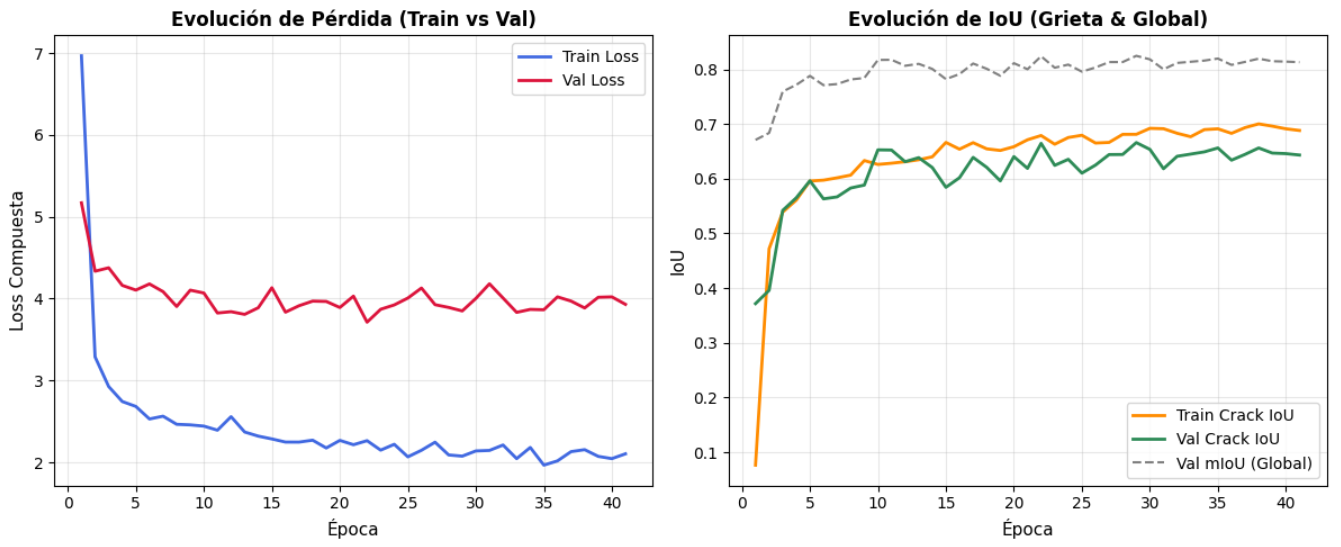
\includegraphics[width=\columnwidth]{figs/loss_iou.png}
\caption{Curvas de evolución del entrenamiento de PIDNet-S sobre DeepCrack: (a) pérdida en entrenamiento y validación, (b) evolución de $mIoU$ global, y (c) progreso del $IoU$ y $F1\text{-Score}$ específico de la clase grieta en validación.}
\label{fig:pidnet_curves}
\end{figure}

\subsection{Comparación Cualitativa}
La evaluación visual de las máscaras predichas revela diferencias marcadas en la morfología de los resultados:
\begin{itemize}
    \item \textbf{Grietas capilares ultrafinas:} UNet++ y PIDNet logran mantener una mejor conectividad estructural. La rama de borde dedicada de PIDNet evita la desconexión de líneas en zonas de bajo contraste con el hormigón.
    \item \textbf{Bordes y suavizado:} YOLOv11-Seg genera contornos más suaves debido a la combinación lineal de prototipos de máscara, lo que en fisuras de trayectoria errática puede derivar en un ligero engrosamiento o pérdida de extremos muy delgados, si bien elimina eficazmente falsos positivos aislados provocados por manchas o sombras en la superficie.
\end{itemize}

\begin{figure}[t]
\centering
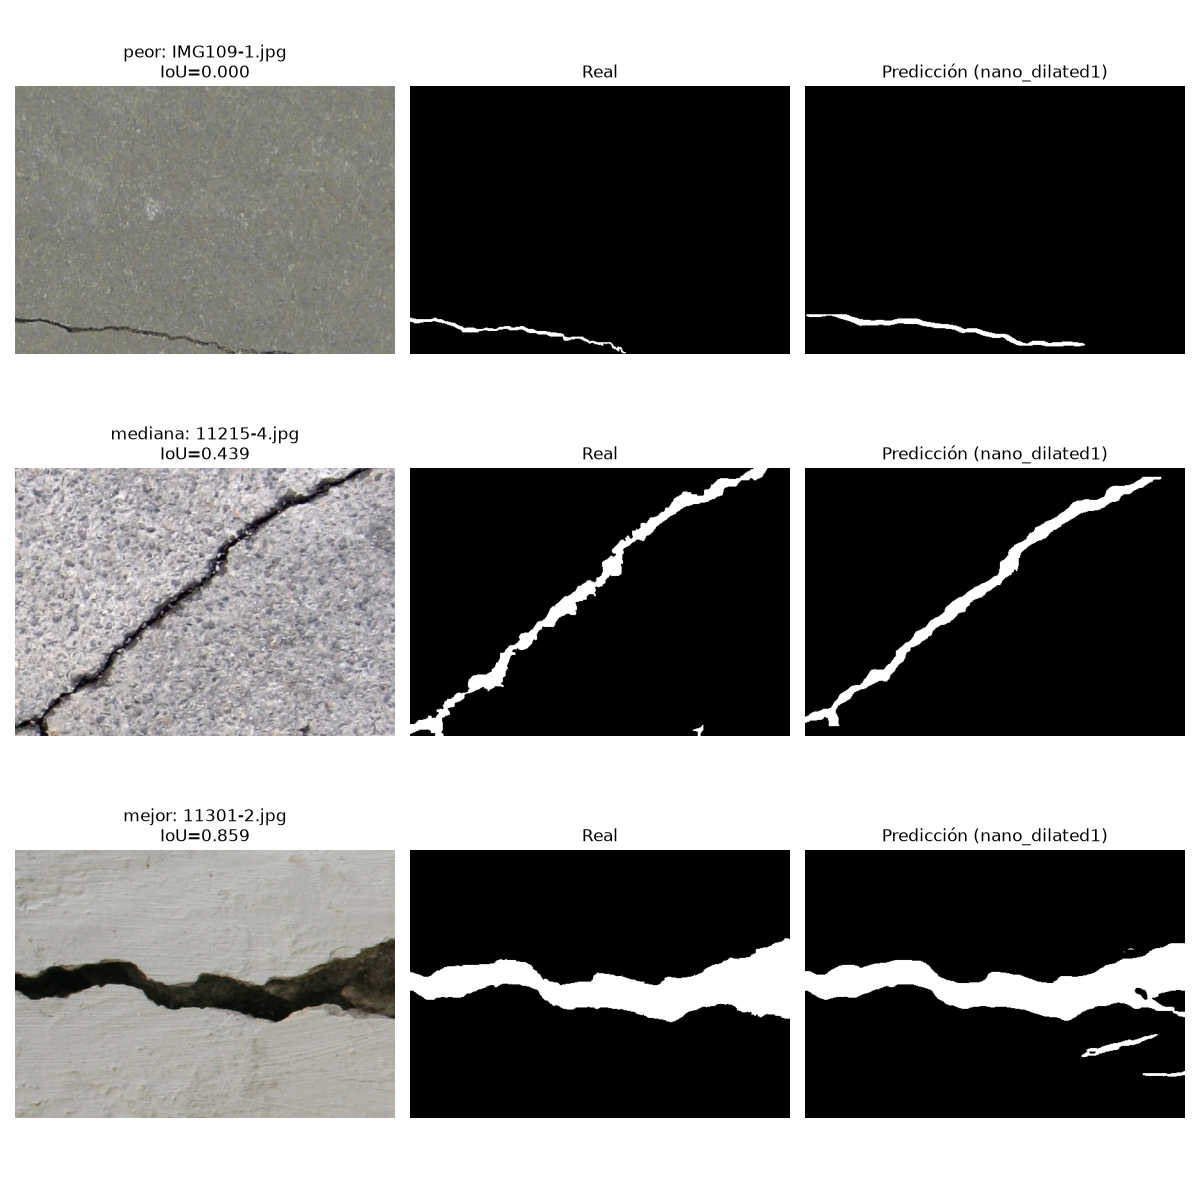
\includegraphics[width=\columnwidth]{figs/semantic_samples_final.png}
\caption{Muestras de evaluación cualitativa sobre el conjunto de prueba de DeepCrack: imagen original, máscara ground-truth y predicciones segmentadas.}
\label{fig:qualitative_samples}
\end{figure}

\subsection{Discusión y Limitaciones Metodológicas}

\subsubsection{Compromiso Precisión vs. Eficiencia (\textit{Trade-off})}
Los resultados validan la existencia de un claro compromiso ingenieril entre costo computacional y fidelidad pixel-wise:
\begin{itemize}
    \item Si el objetivo es la **auditoría estructural \textit{offline} de alta precisión**, donde la exactitud métrica del ancho de grieta es prioritaria y no existen restricciones de tiempo, **UNet++ con atención scSE** representa la opción superior ($IoU_{\text{grieta}} = 0.7314$).
    \item Si el despliegue requiere **monitoreo dinámico en tiempo real** montado en drones (UAVs) o vehículos de inspección con hardware restringido, **PIDNet-S** y **YOLO11-Seg** ofrecen la mejor solución de compromiso, procesando secuencias de video a más de $17-45$~FPS con una pérdida de $IoU$ de apenas 5 a 6 puntos porcentuales respecto a UNet++.
\end{itemize}

\subsubsection{Análisis Crítico de Limitaciones Experimentales}
En consonancia con las pautas de rigor metodológico, es fundamental declarar explícitamente las limitaciones y divergencias técnicas derivadas del trabajo descentralizado del equipo:
\begin{itemize}
    \item \textbf{Diferencias de preprocesamiento y representación:} mientras PIDNet y UNet++ operaron directamente sobre máscaras ráster pixel-wise, YOLOv11 requirió vectorizar componentes conexas a polígonos. Esta transformación introduce un techo teórico intrínseco en la representación geométrica de pequeños vértices.
    \item \textbf{Estrategias de optimización heterogéneas:} cada modelo convergió bajo esquemas de épocas ($50$ en PIDNet, $100$ en UNet++, $200$ en YOLO) y combinaciones de pérdidas disímiles (Boundary CE vs. BCE+Dice vs. YOLO native loss). Si bien esto optimizó el rendimiento individual de cada arquitectura, introduce factores de confusión que impiden aislar estrictamente el impacto exclusivo de la topología de la red.
    \item \textbf{Tamaño del dataset:} con 300 imágenes de entrenamiento, la generalización a escenarios con suciedad extrema o artefactos climáticos fuera del dominio de DeepCrack constituye un desafío a validar en trabajos futuros.
\end{itemize}

\section{Conclusiones Finales}

A partir de la experimentación, análisis cuantitativo y evaluación comparativa de los tres modelos de segmentación semántica sobre el dataset DeepCrack, se derivan las siguientes cinco conclusiones principales:

\begin{enumerate}
    \item \textbf{Fidelidad de segmentación semántica:} UNet++ con codificador ResNet-34 y bloques de atención espacial y de canal (scSE) demostró el desempeño más alto en precisión a nivel de píxel ($IoU_{\text{grieta}} = 0.7314$, $mIoU = 0.8588$), confirmando la superioridad de las conexiones densas anidadas para preservar la continuidad en fisuras estructurales complejas.
    \item \textbf{Viabilidad operativa en tiempo real:} PIDNet-S y YOLO11-Seg probaron ser alternativas altamente eficientes para procesamiento en tiempo real, alcanzando tasas de $17.04$~FPS y hasta $>45$~FPS respectivamente sobre GPU NVIDIA T4, lo que habilita su despliegue directo en flujos de video continuo.
    \item \textbf{Eficacia de la supervisión de contornos (PIDNet):} La incorporación de una rama derivativa de bordes explícita modulada mediante pérdida \textit{Boundary-Aware} permitió a PIDNet alcanzar un $IoU_{\text{grieta}}$ de $0.6660$ con una reducción del 48\% en la latencia respecto a UNet++, evidenciando la efectividad de guiar la segmentación de estructuras delgadas mediante información de alta frecuencia.
    \item \textbf{Criterios de selección para ingeniería civil:} Se establece una pauta de selección clara según el caso de uso: UNet++ se consolida como el modelo óptimo para inspecciones estáticas y auditorías forenses de alta precisión (\textit{offline}), mientras que PIDNet y YOLOv11 son los modelos indicados para inspecciones dinámicas y patrullajes autónomos mediante drones (UAVs) o vehículos terrestres.
    \item \textbf{Lecciones metodológicas y trabajo futuro:} El estudio demostró la importancia crítica de unificar formatos de entrada y criterios de evaluación. Como trabajo futuro, se proyecta integrar técnicas de cuantificación métrica del ancho de grieta en milímetros combinando la segmentación con parámetros de cámara UAV~\cite{liu2025crack}, así como la cuantización a FP16/INT8 mediante TensorRT para su implementación en dispositivos embebidos de bajo consumo (e.g., NVIDIA Jetson).
\end{enumerate}

\begin{thebibliography}{00}
\bibitem{kaveh2024recent} A. Kaveh and M. Alhajj, ``Recent advances in crack detection technologies for structures,'' \emph{Frontiers in Built Environment}, vol. 10, p. 1321634, 2024.
\bibitem{perry2020streamlined} B. J. Perry, Y. Guo, R. Atadero, and J. W. van de Lindt, ``Streamlined bridge inspection system utilizing unmanned aerial vehicles (UAVs) and machine learning,'' \emph{Measurement}, vol. 164, p. 108048, 2020.
\bibitem{liu2025crack} Z.-L. Liu, A. Zhou, X.-R. Ran, Y.-P. Wu, W.-G. Zhao, and H. Zhang, ``A crack detection and quantification method using matched filter and photograph reconstruction,'' \emph{Scientific Reports}, vol. 15, no. 1, p. 25266, 2025.
\bibitem{haciefendioglu2022concrete} K. Hac{\i}efendio{\u{g}}lu and H. B. Ba{\c{s}}a{\u{g}}a, ``Concrete road crack detection using deep learning-based Faster R-CNN method,'' \emph{Iranian Journal of Science and Technology, Transactions of Civil Engineering}, vol. 46, no. 2, pp. 1025--1036, 2022.
\bibitem{zhang2025accuracy} J. Zhang, Z. V. Beliaeva, and Y. Huang, ``Accuracy--efficiency trade-off: Optimizing YOLOv8 for structural crack detection,'' \emph{Sensors}, vol. 25, no. 13, p. 3873, 2025.
\bibitem{liu2019deepcrack} Y. Liu, J. Yao, X. Lu, R. Xie, and L. Li, ``DeepCrack: A deep hierarchical feature learning architecture for crack segmentation,'' \emph{Neurocomputing}, vol. 338, pp. 139--153, 2019.
\bibitem{zhou2018unetplusplus} Z. Zhou, M. M. R. Siddiquee, N. Tajbakhsh, and J. Liang, ``UNet++: A nested U-Net architecture for medical image segmentation,'' in \emph{Deep Learning in Medical Image Analysis and Multimodal Learning for Clinical Decision Support}, Springer, 2018, pp. 3--11.
\bibitem{xu2023pidnet} J. Xu, Z. Xiong, and S. P. Bhattacharyya, ``PIDNet: A real-time semantic segmentation network inspired by PID controllers,'' in \emph{Proceedings of the IEEE/CVF International Conference on Computer Vision (ICCV)}, 2023, pp. 19529--19539.
\bibitem{kahn2024yolo11} G. Jocher, A. Chaurasia, and J. Qiu, ``Ultralytics YOLO11,'' 2024. [Online]. Available: \url{https://github.com/ultralytics/ultralytics}
\bibitem{hu2019topology} C. Hu, D. Peng, P. Guan, et al., ``Topology-preserving deep image segmentation,'' in \emph{Advances in Neural Information Processing Systems (NeurIPS)}, vol. 32, 2019.
\bibitem{wang2024pavement} Y. Wang, et al., ``Pavement fatigue crack detection and severity classification based on convolutional neural network,'' \emph{arXiv preprint arXiv:2407.16021}, 2024.
\end{thebibliography}

\end{document}
